\documentclass{standalone}
\usepackage{tikz}
\usetikzlibrary{patterns}
\usetikzlibrary{positioning}
\usetikzlibrary{patterns, positioning}
\usetikzlibrary{shapes.misc}
\usepackage[outline]{contour}
\contourlength{1.5pt} 
\usepackage[sfdefault]{ClearSans}

\begin{document}
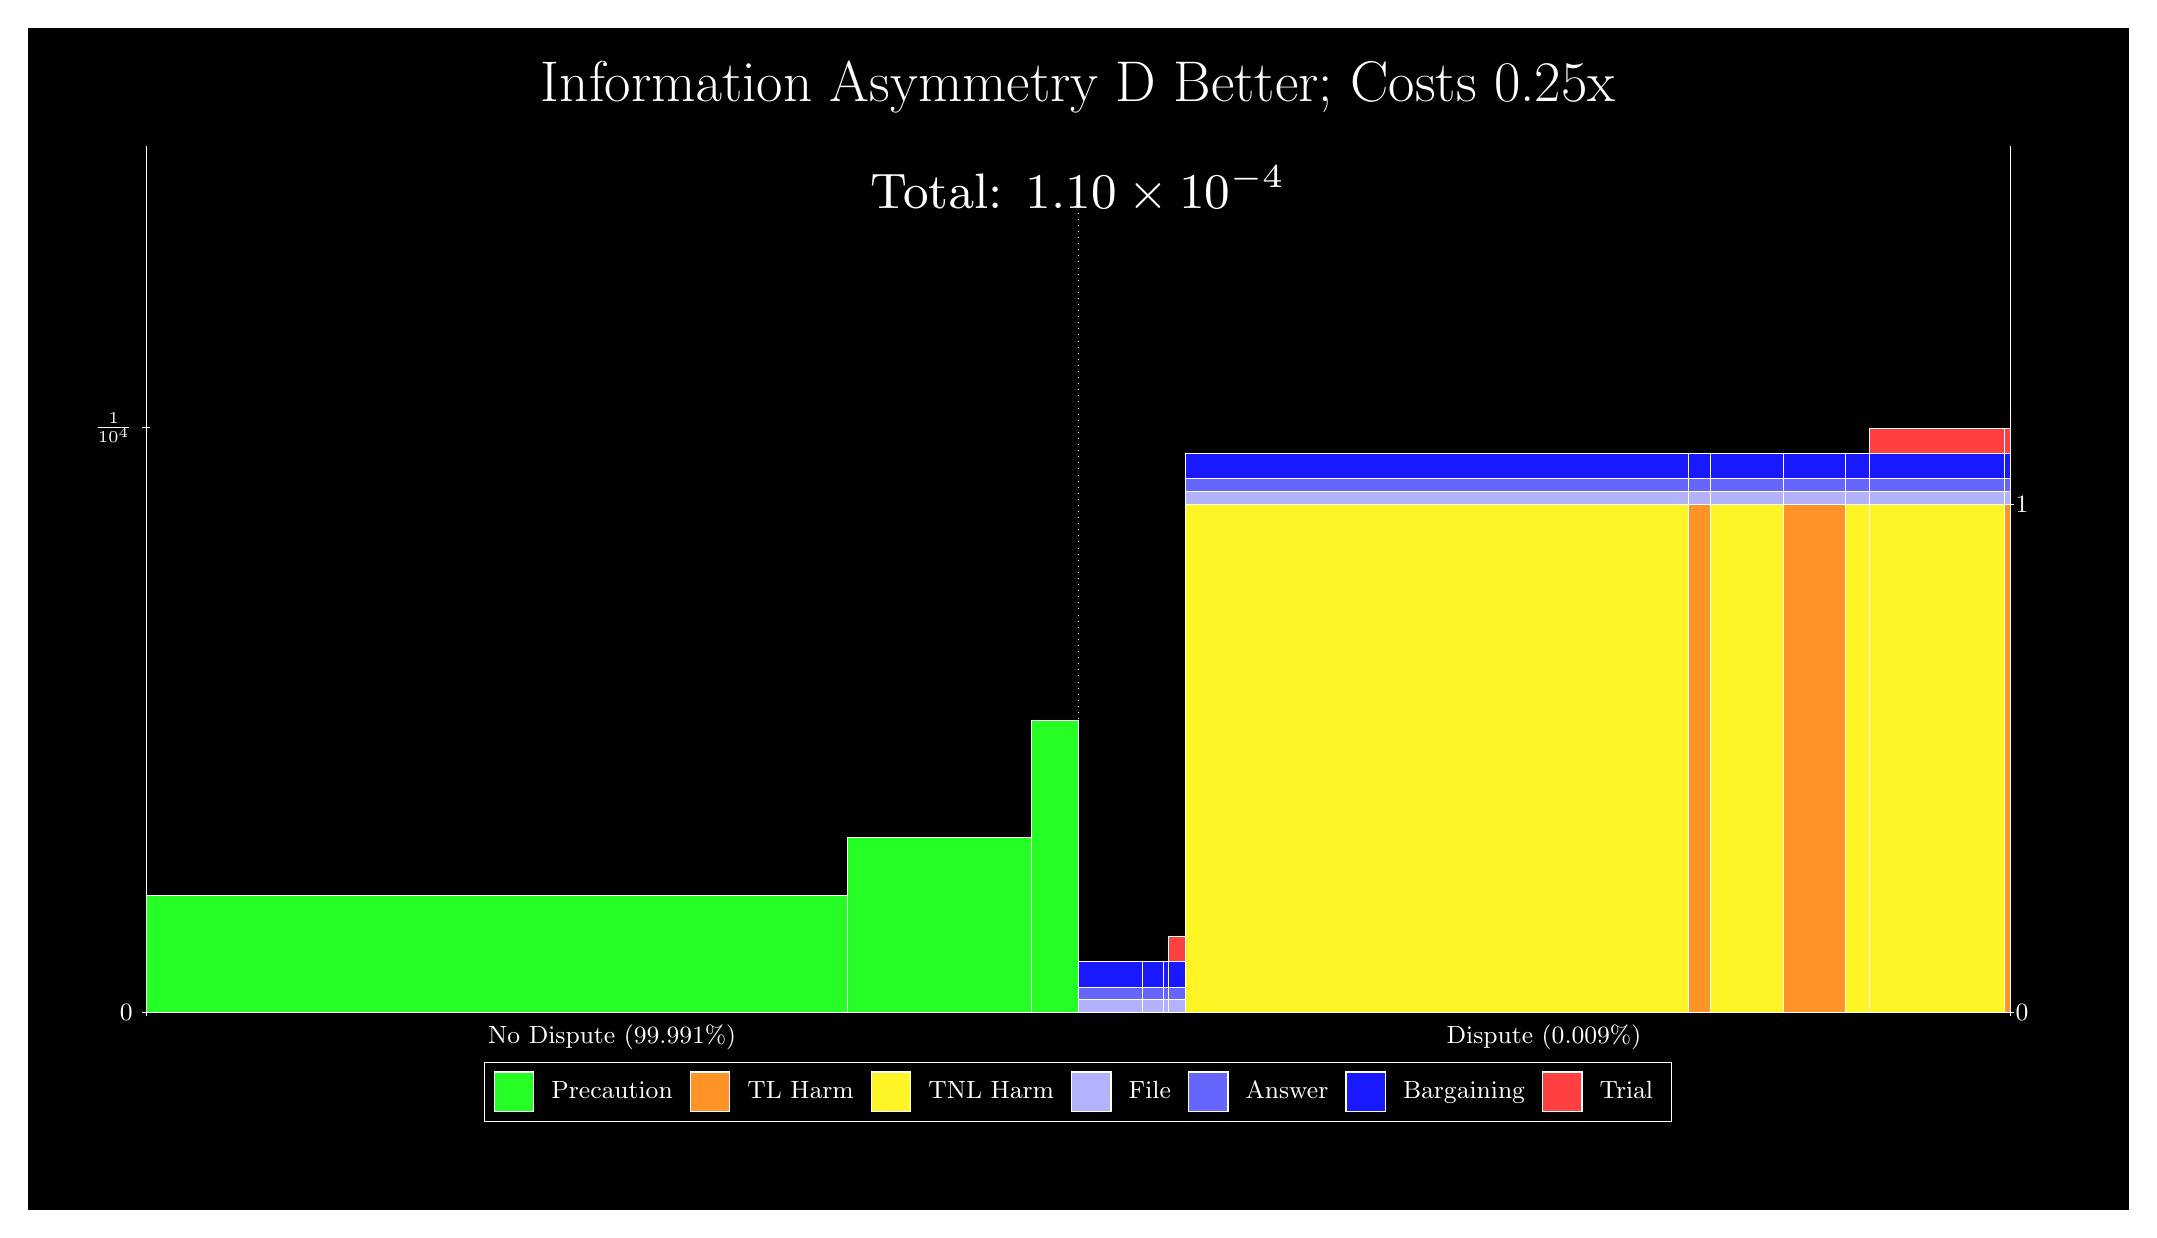
\begin{tikzpicture}
\draw[fill=black] (0,0) rectangle (26.667,15);
\draw[draw=none,text=white] (0,13.5) rectangle (26.667,15) node[midway] {\huge Information Asymmetry D Better; Costs 0.25x};
\draw[fill=green!85,draw=white,very thin] (1.5,2.5) rectangle (10.403,3.9854);
\draw[fill=green!85,draw=white,very thin] (10.403,2.5) rectangle (12.739,4.7282);
\draw[fill=green!85,draw=white,very thin] (12.739,2.5) rectangle (13.333,6.2136);
\draw[fill=green!85,draw=white,very thin] (13.333,2.5) rectangle (14.143,2.5001);
\draw[fill=blue!30,draw=white,very thin] (13.333,2.5001) rectangle (14.143,2.6615);
\draw[fill=blue!60,draw=white,very thin] (13.333,2.6615) rectangle (14.143,2.823);
\draw[fill=blue!90,draw=white,very thin] (13.333,2.823) rectangle (14.143,3.1458);
\draw[fill=green!85,draw=white,very thin] (14.143,2.5) rectangle (14.413,2.5002);
\draw[fill=blue!30,draw=white,very thin] (14.143,2.5002) rectangle (14.413,2.6616);
\draw[fill=blue!60,draw=white,very thin] (14.143,2.6616) rectangle (14.413,2.823);
\draw[fill=blue!90,draw=white,very thin] (14.143,2.823) rectangle (14.413,3.1459);
\draw[fill=green!85,draw=white,very thin] (14.413,2.5) rectangle (14.482,2.5003);
\draw[fill=blue!30,draw=white,very thin] (14.413,2.5003) rectangle (14.482,2.6617);
\draw[fill=blue!60,draw=white,very thin] (14.413,2.6617) rectangle (14.482,2.8232);
\draw[fill=blue!90,draw=white,very thin] (14.413,2.8232) rectangle (14.482,3.146);
\draw[fill=green!85,draw=white,very thin] (14.482,2.5) rectangle (14.695,2.5001);
\draw[fill=blue!30,draw=white,very thin] (14.482,2.5001) rectangle (14.695,2.6615);
\draw[fill=blue!60,draw=white,very thin] (14.482,2.6615) rectangle (14.695,2.823);
\draw[fill=blue!90,draw=white,very thin] (14.482,2.823) rectangle (14.695,3.1458);
\draw[fill=red!75,draw=white,very thin] (14.482,3.1458) rectangle (14.695,3.4686);
\draw[fill=green!85,draw=white,very thin] (14.695,2.5) rectangle (21.085,2.5001);
\draw[fill=yellow!85,draw=white,very thin] (14.695,2.5001) rectangle (21.085,8.9569);
\draw[fill=blue!30,draw=white,very thin] (14.695,8.9569) rectangle (21.085,9.1183);
\draw[fill=blue!60,draw=white,very thin] (14.695,9.1183) rectangle (21.085,9.2797);
\draw[fill=blue!90,draw=white,very thin] (14.695,9.2797) rectangle (21.085,9.6025);
\draw[fill=green!85,draw=white,very thin] (21.085,2.5) rectangle (21.362,2.5001);
\draw[fill=orange!85,draw=white,very thin] (21.085,2.5001) rectangle (21.362,8.9569);
\draw[fill=blue!30,draw=white,very thin] (21.085,8.9569) rectangle (21.362,9.1183);
\draw[fill=blue!60,draw=white,very thin] (21.085,9.1183) rectangle (21.362,9.2797);
\draw[fill=blue!90,draw=white,very thin] (21.085,9.2797) rectangle (21.362,9.6025);
\draw[fill=green!85,draw=white,very thin] (21.362,2.5) rectangle (22.293,2.5002);
\draw[fill=yellow!85,draw=white,very thin] (21.362,2.5002) rectangle (22.293,8.9569);
\draw[fill=blue!30,draw=white,very thin] (21.362,8.9569) rectangle (22.293,9.1183);
\draw[fill=blue!60,draw=white,very thin] (21.362,9.1183) rectangle (22.293,9.2798);
\draw[fill=blue!90,draw=white,very thin] (21.362,9.2798) rectangle (22.293,9.6026);
\draw[fill=green!85,draw=white,very thin] (22.293,2.5) rectangle (23.082,2.5002);
\draw[fill=orange!85,draw=white,very thin] (22.293,2.5002) rectangle (23.082,8.9569);
\draw[fill=blue!30,draw=white,very thin] (22.293,8.9569) rectangle (23.082,9.1183);
\draw[fill=blue!60,draw=white,very thin] (22.293,9.1183) rectangle (23.082,9.2798);
\draw[fill=blue!90,draw=white,very thin] (22.293,9.2798) rectangle (23.082,9.6026);
\draw[fill=green!85,draw=white,very thin] (23.082,2.5) rectangle (23.383,2.5003);
\draw[fill=yellow!85,draw=white,very thin] (23.082,2.5003) rectangle (23.383,8.9571);
\draw[fill=blue!30,draw=white,very thin] (23.082,8.9571) rectangle (23.383,9.1185);
\draw[fill=blue!60,draw=white,very thin] (23.082,9.1185) rectangle (23.383,9.2799);
\draw[fill=blue!90,draw=white,very thin] (23.082,9.2799) rectangle (23.383,9.6027);
\draw[fill=green!85,draw=white,very thin] (23.383,2.5) rectangle (25.097,2.5001);
\draw[fill=yellow!85,draw=white,very thin] (23.383,2.5001) rectangle (25.097,8.9569);
\draw[fill=blue!30,draw=white,very thin] (23.383,8.9569) rectangle (25.097,9.1183);
\draw[fill=blue!60,draw=white,very thin] (23.383,9.1183) rectangle (25.097,9.2797);
\draw[fill=blue!90,draw=white,very thin] (23.383,9.2797) rectangle (25.097,9.6025);
\draw[fill=red!75,draw=white,very thin] (23.383,9.6025) rectangle (25.097,9.9254);
\draw[fill=green!85,draw=white,very thin] (25.097,2.5) rectangle (25.167,2.5001);
\draw[fill=orange!85,draw=white,very thin] (25.097,2.5001) rectangle (25.167,8.9569);
\draw[fill=blue!30,draw=white,very thin] (25.097,8.9569) rectangle (25.167,9.1183);
\draw[fill=blue!60,draw=white,very thin] (25.097,9.1183) rectangle (25.167,9.2797);
\draw[fill=blue!90,draw=white,very thin] (25.097,9.2797) rectangle (25.167,9.6025);
\draw[fill=red!75,draw=white,very thin] (25.097,9.6025) rectangle (25.167,9.9254);
\node[font=\small,text=white,anchor=north,scale=2] at (13.333, 13.5) {Total: $1.10\times 10^{-4}$};
\draw[white,very thin] (1.5,2.5) -- (1.5,13.5);
\draw[white,very thin] (1.45,2.5) -- (1.55,2.5);
\node[font=\small,text=white, anchor=east] at (1.45, 2.5) {0};
\draw[white,very thin] (1.45,9.9272) -- (1.55,9.9272);
\node[font=\small,text=white, anchor=east] at (1.45, 9.9272) {$\frac{1}{10^{4}}$};

\draw[white,dotted,very thin] (13.333,2.83) -- (13.333,13.17);
\draw[white,very thin] (25.167,2.5) -- (25.167,13.5);
\draw[white,very thin] (25.117,2.5) -- (25.217,2.5);
\node[font=\small,text=white, anchor=west] at (25.117, 2.5) {0};
\draw[white,very thin] (25.117,8.9567) -- (25.217,8.9567);
\node[font=\small,text=white, anchor=west] at (25.117, 8.9567) {1};

\draw[white,very thin] (1.5,2.5) -- (25.167,2.5);
\draw[white,very thin] (1.5,2.45) -- (1.5,2.55);
\node[font=\small,text=white, anchor=north] at (1.5, 2.45) {};
\draw[white,very thin] (25.167,2.45) -- (25.167,2.55);
\node[font=\small,text=white, anchor=north] at (25.167, 2.45) {};

\node[font=\small,text=white,anchor=south] at (7.4167, 1.9) {No\ Dispute\ (99.991\%)};
\node[font=\small,text=white,anchor=south] at (19.25, 1.9) {Dispute\ (0.009\%)};
\draw (13.3333,2.5) node (B) {};
\begin{scope}[align=center]
\matrix[scale=0.5,draw=white,below=0.5cm of B,nodes={draw},column sep=0.1cm]{
\node[rectangle,draw,minimum width=0.5cm,minimum height=0.5cm,fill=green!85]{}; & \node[draw=none,font=\small,text=white]{Precaution}; &
\node[rectangle,draw,minimum width=0.5cm,minimum height=0.5cm,fill=orange!85]{}; & \node[draw=none,font=\small,text=white]{TL Harm}; &
\node[rectangle,draw,minimum width=0.5cm,minimum height=0.5cm,fill=yellow!85]{}; & \node[draw=none,font=\small,text=white]{TNL Harm}; &
\node[rectangle,draw,minimum width=0.5cm,minimum height=0.5cm,fill=blue!30]{}; & \node[draw=none,font=\small,text=white]{File}; &
\node[rectangle,draw,minimum width=0.5cm,minimum height=0.5cm,fill=blue!60]{}; & \node[draw=none,font=\small,text=white]{Answer}; &
\node[rectangle,draw,minimum width=0.5cm,minimum height=0.5cm,fill=blue!90]{}; & \node[draw=none,font=\small,text=white]{Bargaining}; &
\node[rectangle,draw,minimum width=0.5cm,minimum height=0.5cm,fill=red!75]{}; & \node[draw=none,font=\small,text=white]{Trial}; \\\\
};\end{scope}

\end{tikzpicture}
\end{document}